\section{Results}
\subsection{Testing system} \label{sec:system}
All experiments are executed on a machine with the following specifications:
\begin{itemize}
  \item GPU: nVidia GTX 570 (480 core)
  \item CPU: Intel 8 core cpu
\end{itemize}

\subsection{Comparison}
	Figure~\ref{fig:results} gives a comparison for both the time and accurary of the CPU and GPU versions of the program.
	Note that the models have a large influence on which of the two is faster.
	
	In the ideal case, the output of the GPU program is identical to the output of the CPU program.
	We suspect that the missing collisions in a number of models is due to our lower \texttt{maxSize} setting.
	We note that the models that cause our algorithm to exhibit a very low accuracy are faster on the GPU than on the CPU.
	
	These results consist of 200 samples per version, so 400 versions per model.
	Batching was not used here since none of the models required it and it in fact slowed down the GPU version considerably.
	
	\begin{figure}
		\centering
		\begin{subfigure}[b]{0.45\textwidth}
			\begin{subfigure}[b]{0.45\textwidth}
				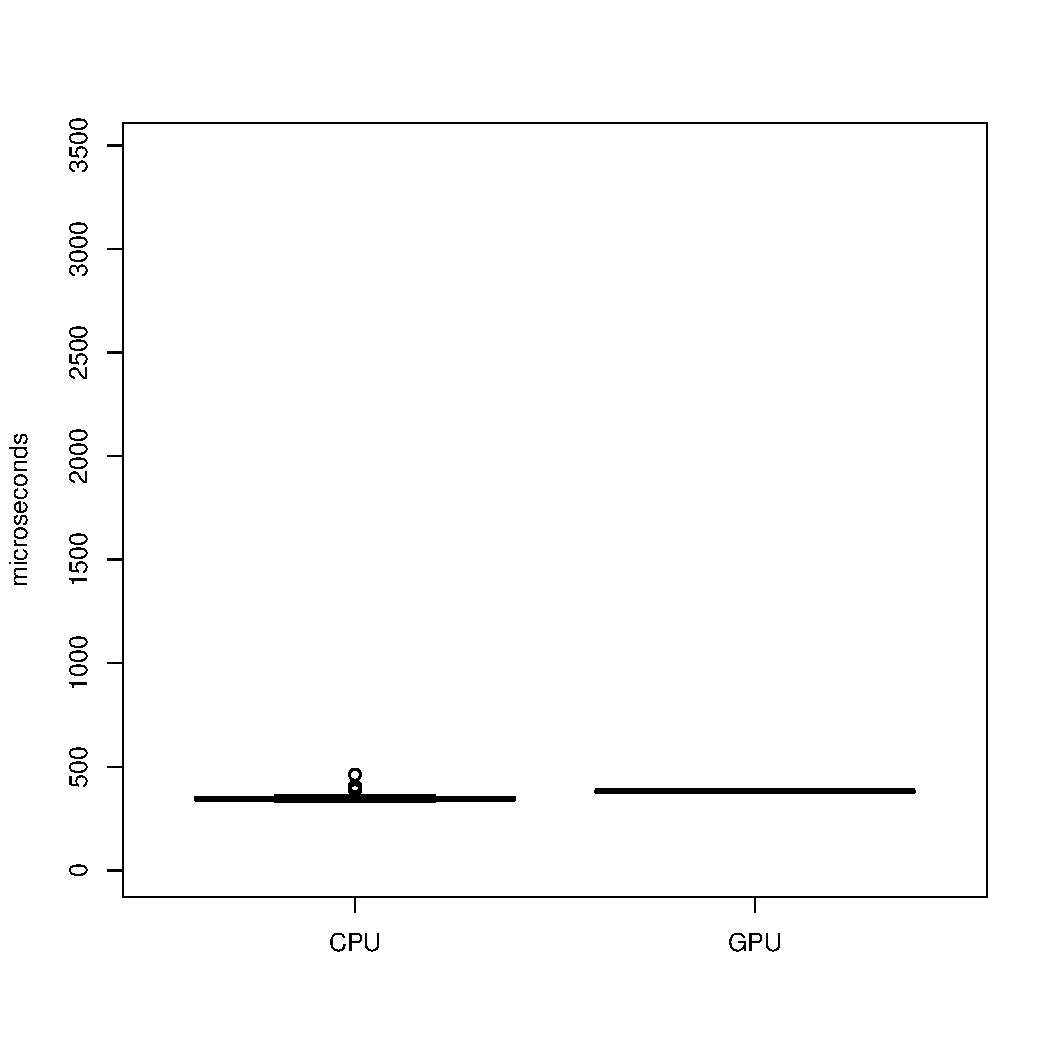
\includegraphics[width=\textwidth]{results/time/armadillo}
			\end{subfigure}
			~%
			\begin{subfigure}[b]{0.45\textwidth}
				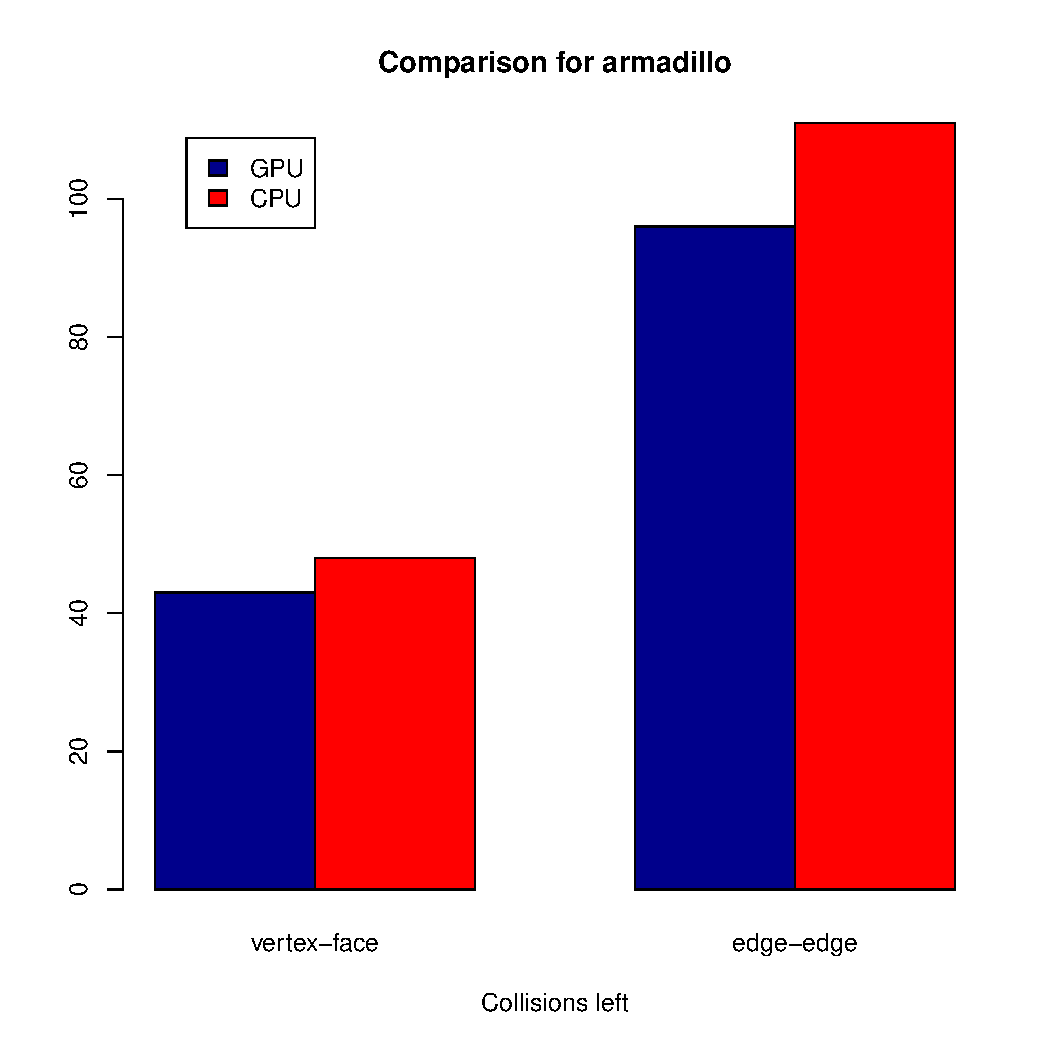
\includegraphics[width=\textwidth]{results/correctness/armadillo}
			\end{subfigure}
			\caption{Model \texttt{armadillo\_10000.txt}}
		\end{subfigure}
		~%
		\begin{subfigure}[b]{0.45\textwidth}
			\begin{subfigure}[b]{0.45\textwidth}
				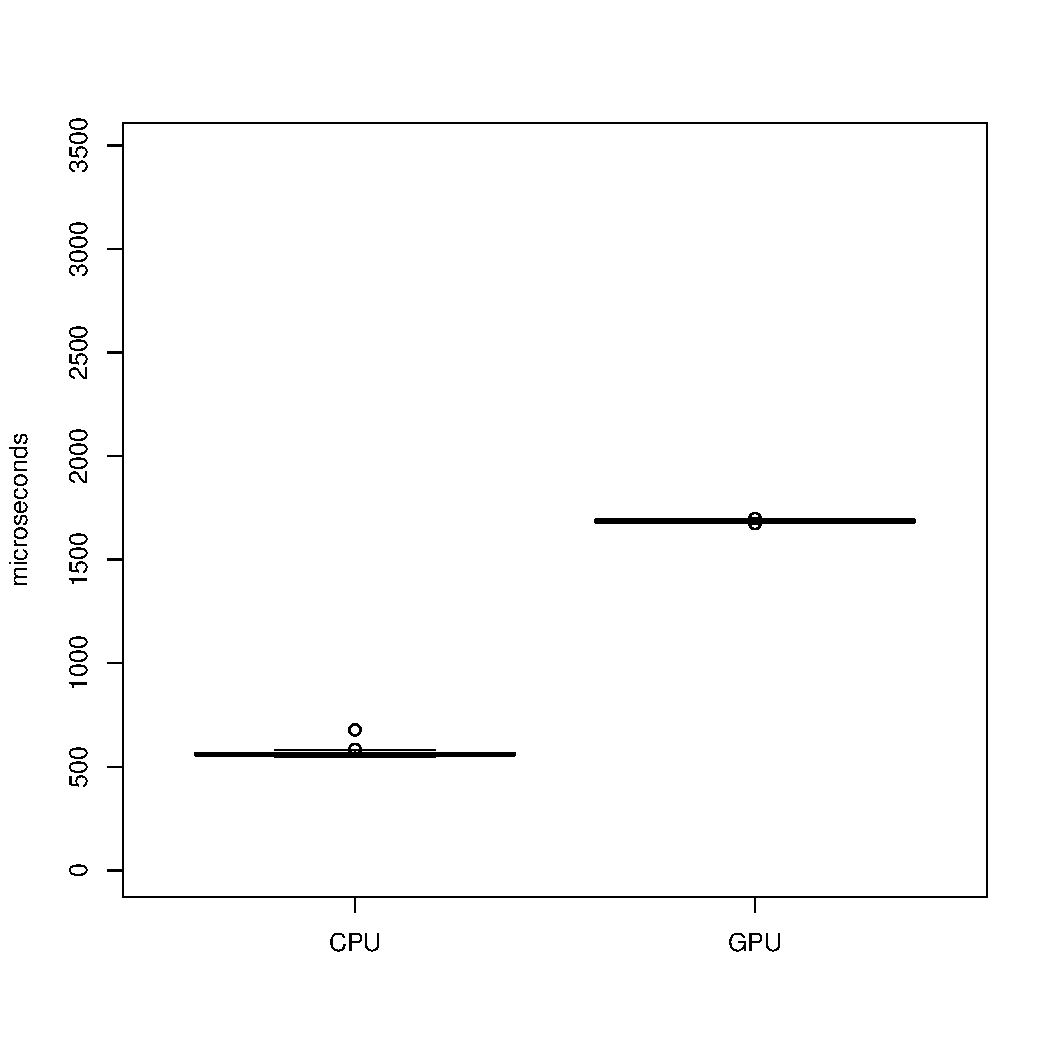
\includegraphics[width=\textwidth]{results/time/asiandragon9a_50000}
			\end{subfigure}
			~%
			\begin{subfigure}[b]{0.45\textwidth}
				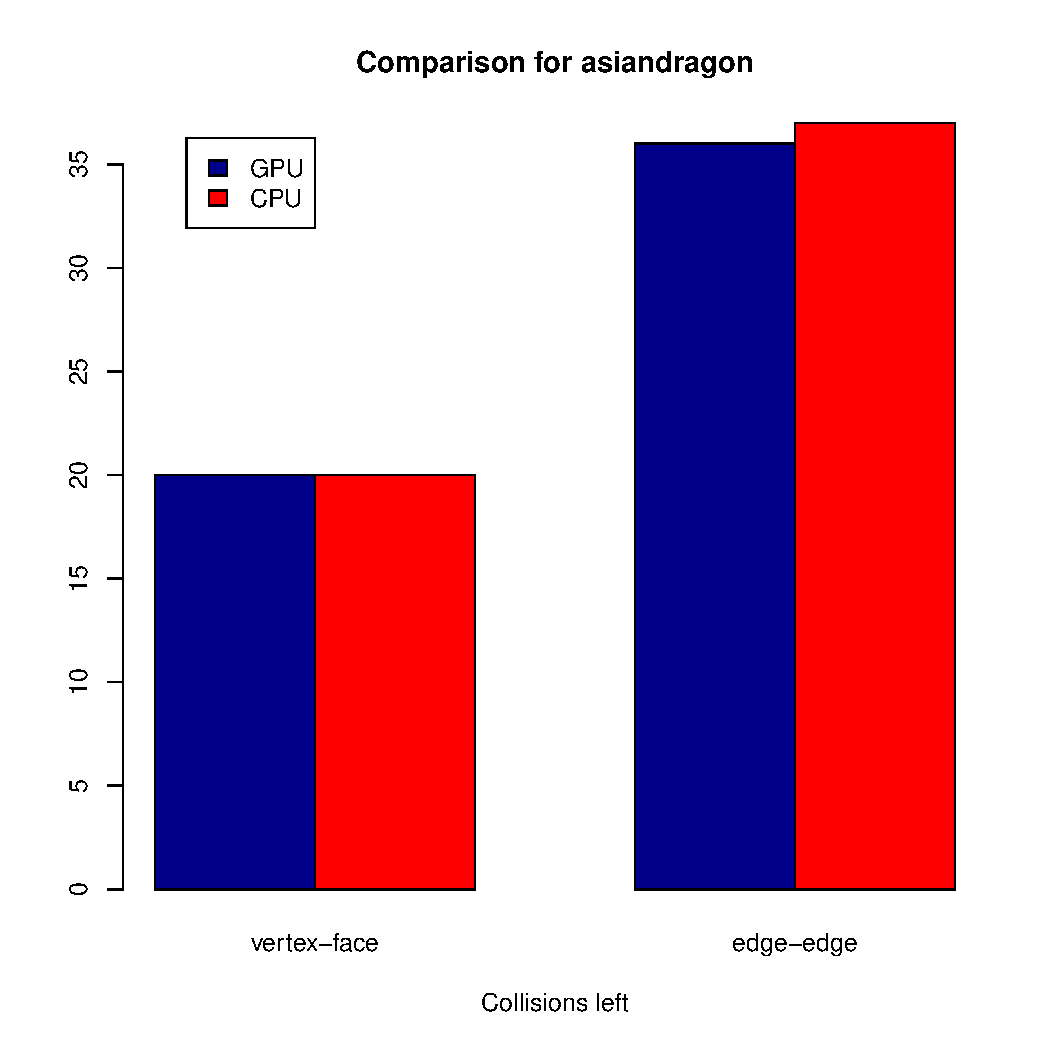
\includegraphics[width=\textwidth]{results/correctness/asiandragon9a_50000}
			\end{subfigure}
			\caption{Model \texttt{asiandragon9a\_50000.txt}}
		\end{subfigure}
		
		\begin{subfigure}[b]{0.45\textwidth}
			\begin{subfigure}[b]{0.45\textwidth}
				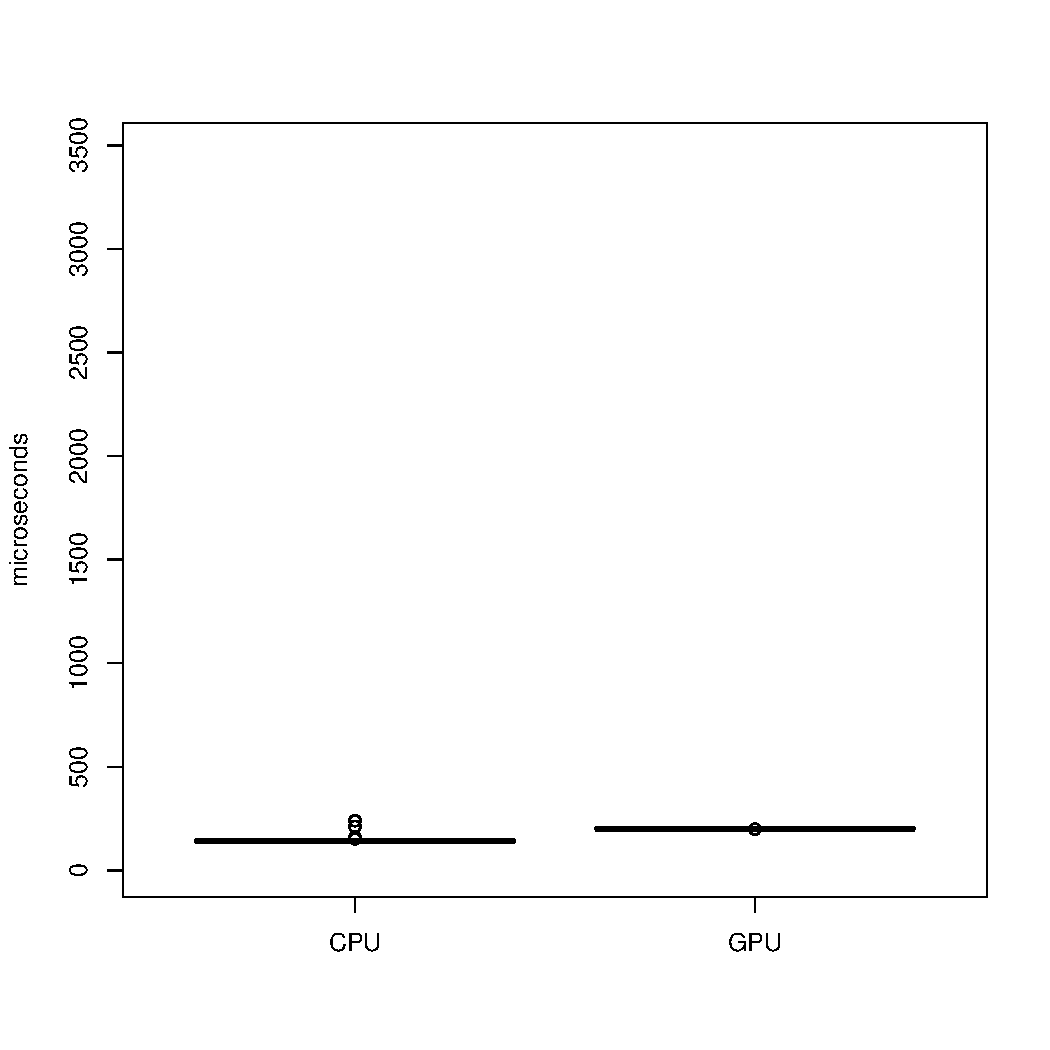
\includegraphics[width=\textwidth]{results/time/bunny}
			\end{subfigure}
			~%
			\begin{subfigure}[b]{0.45\textwidth}
				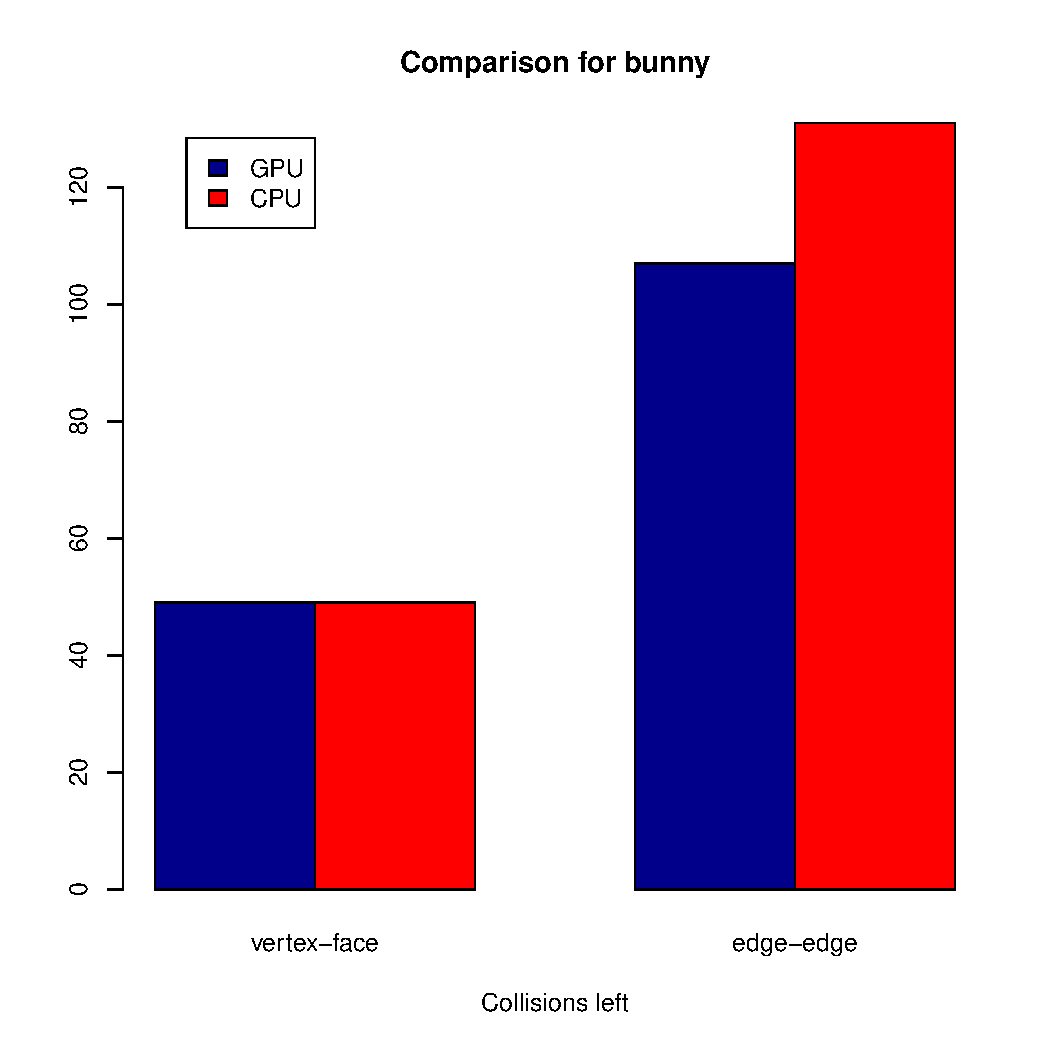
\includegraphics[width=\textwidth]{results/correctness/bunny}
			\end{subfigure}
			\caption{Model \texttt{bunny.txt}}
		\end{subfigure}
		~%
		\begin{subfigure}[b]{0.45\textwidth}
			\begin{subfigure}[b]{0.45\textwidth}
				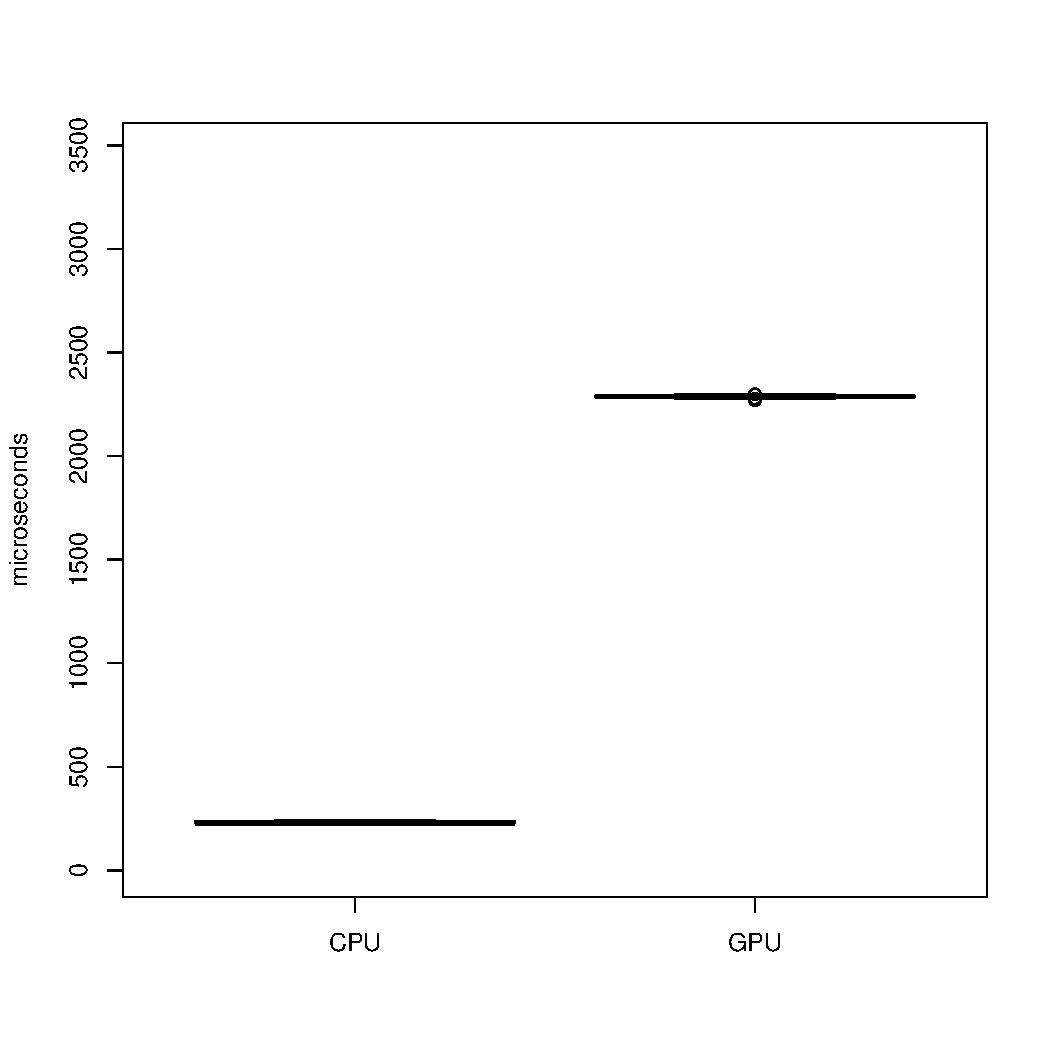
\includegraphics[width=\textwidth]{results/time/bunny2}
			\end{subfigure}
			~%
			\begin{subfigure}[b]{0.45\textwidth}
				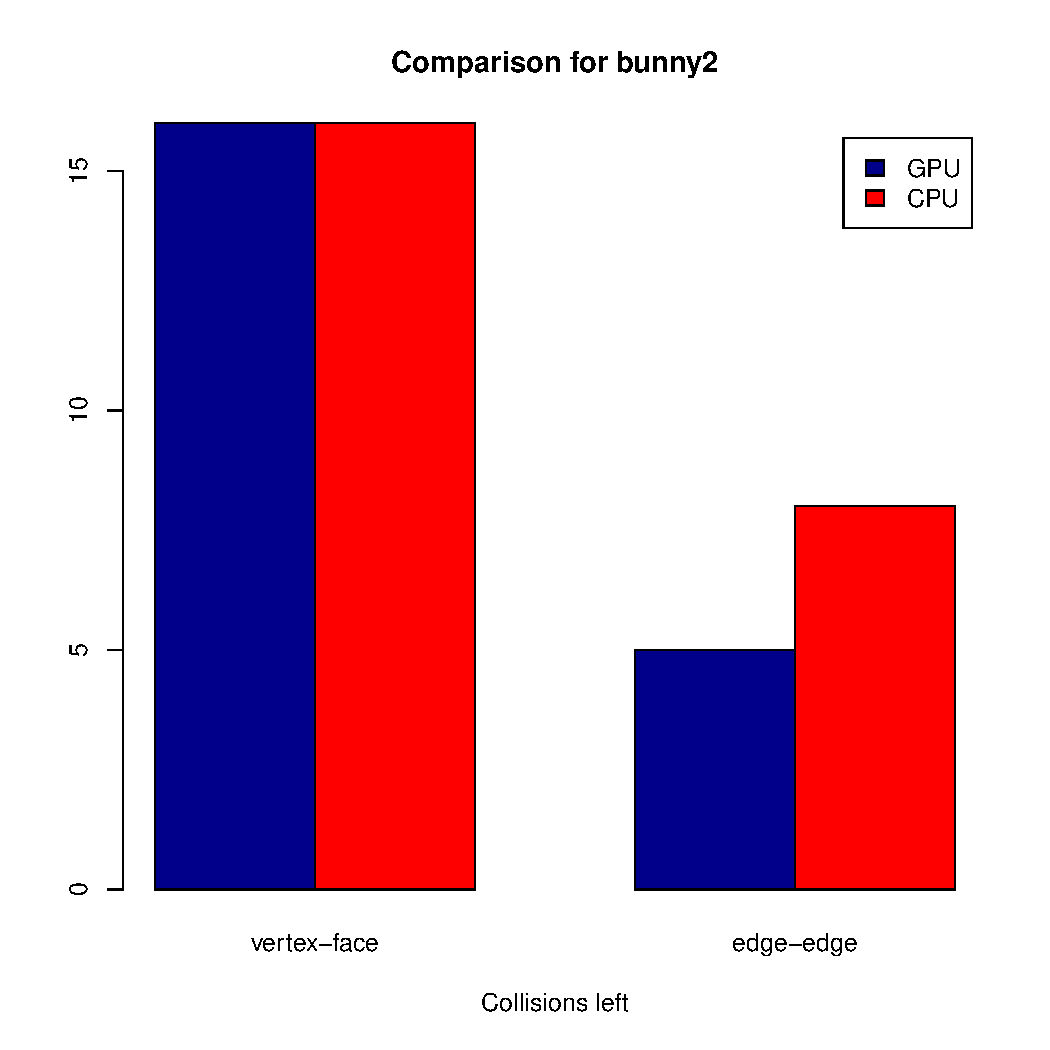
\includegraphics[width=\textwidth]{results/correctness/bunny2}
			\end{subfigure}
			\caption{Model \texttt{bunny2.txt}}
		\end{subfigure}
		
		\begin{subfigure}[b]{0.45\textwidth}
			\begin{subfigure}[b]{0.45\textwidth}
				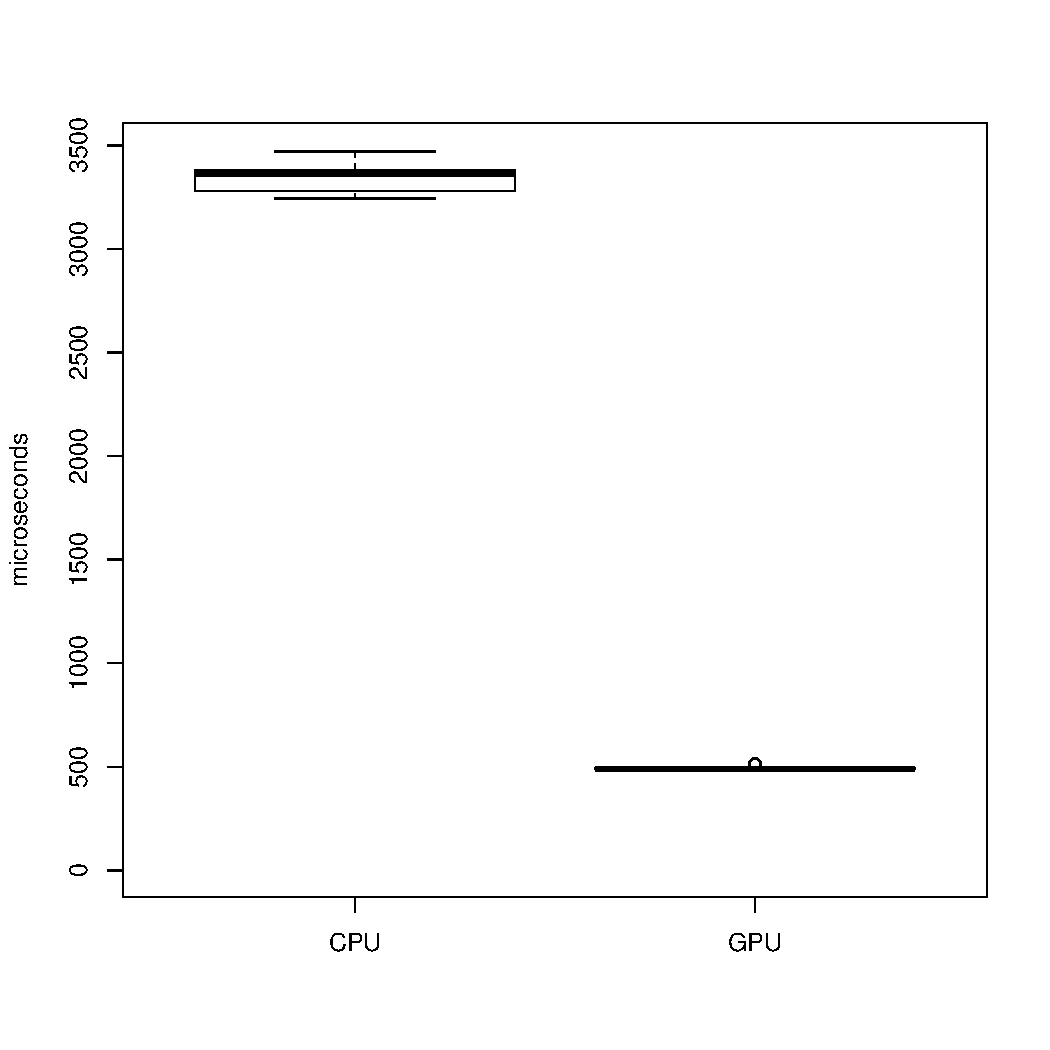
\includegraphics[width=\textwidth]{results/time/lucy_5000}
			\end{subfigure}
			~%
			\begin{subfigure}[b]{0.45\textwidth}
				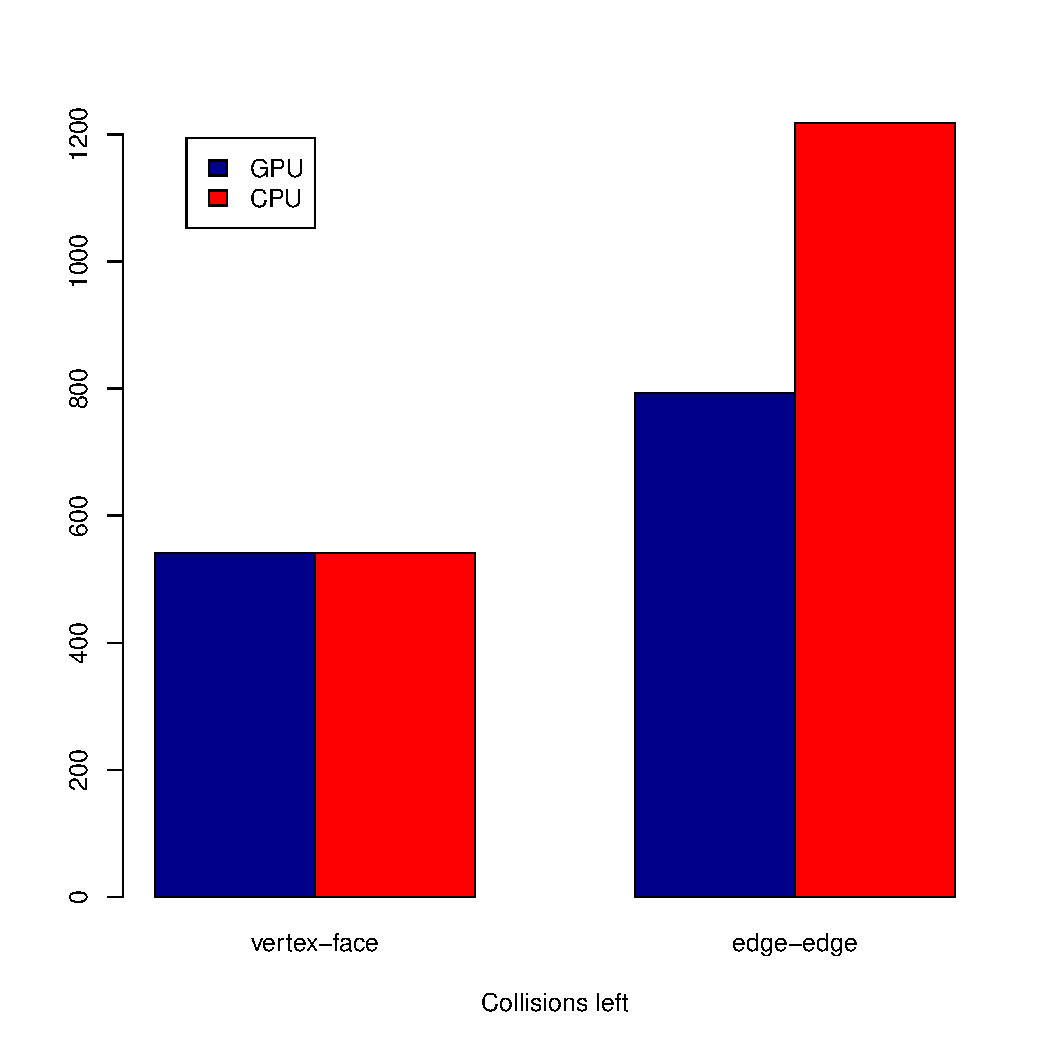
\includegraphics[width=\textwidth]{results/correctness/lucy_5000}
			\end{subfigure}
			\caption{Model \texttt{lucy\_5000.txt}}
		\end{subfigure}
		~%
		\begin{subfigure}[b]{0.45\textwidth}
			\begin{subfigure}[b]{0.45\textwidth}
				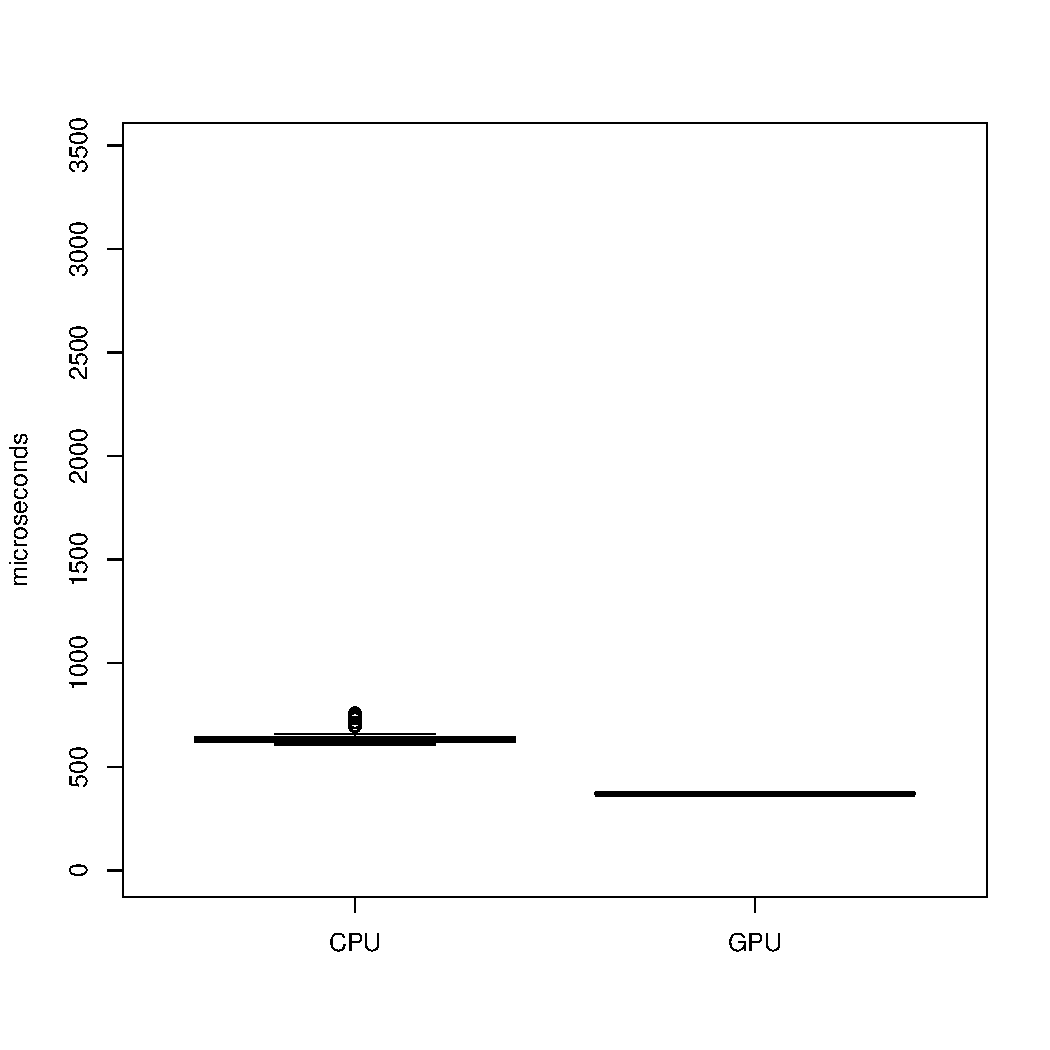
\includegraphics[width=\textwidth]{results/time/neptune_10000}
			\end{subfigure}
			~%
			\begin{subfigure}[b]{0.45\textwidth}
				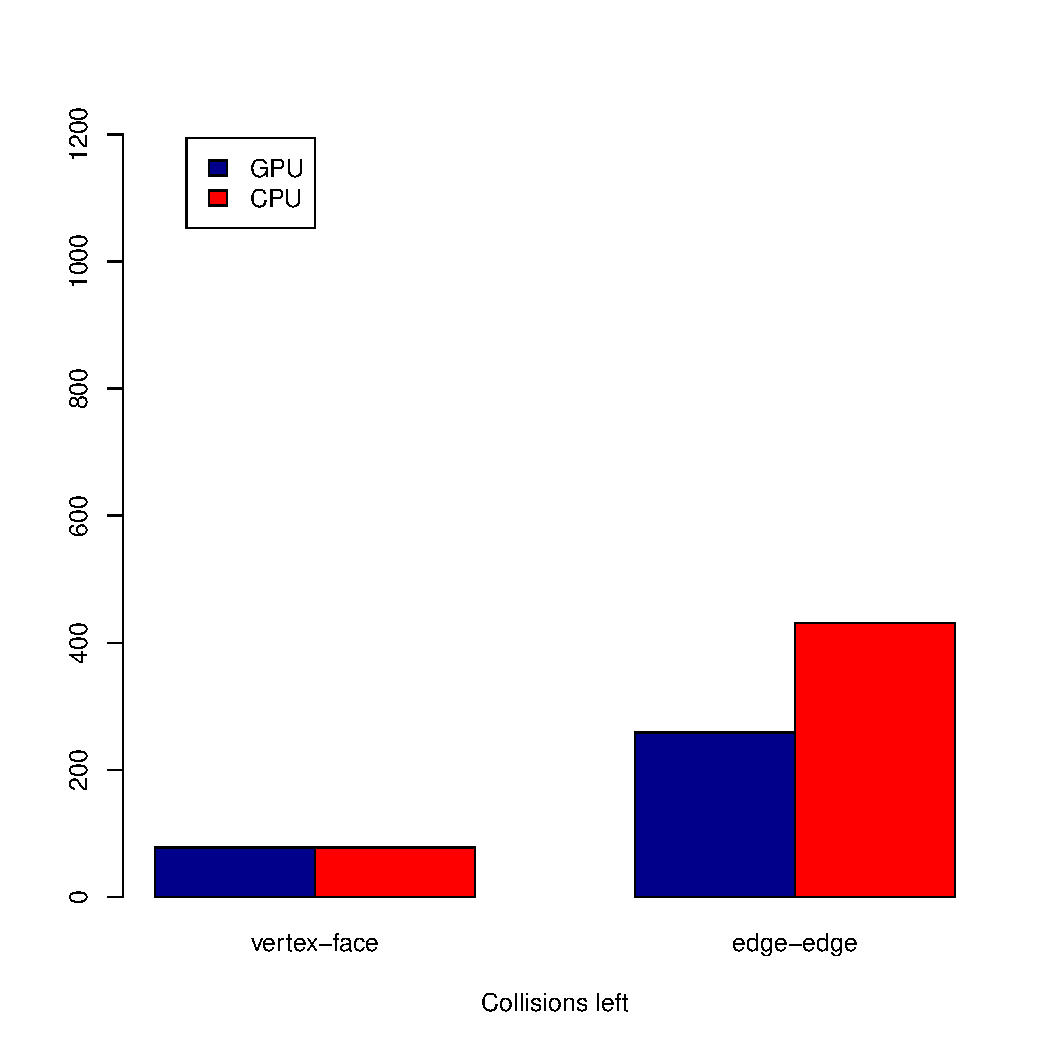
\includegraphics[width=\textwidth]{results/correctness/neptune_10000}
			\end{subfigure}
			\caption{Model \texttt{neptune\_10000.txt}}
		\end{subfigure}
		
		\begin{subfigure}[b]{0.45\textwidth}
			\begin{subfigure}[b]{0.45\textwidth}
				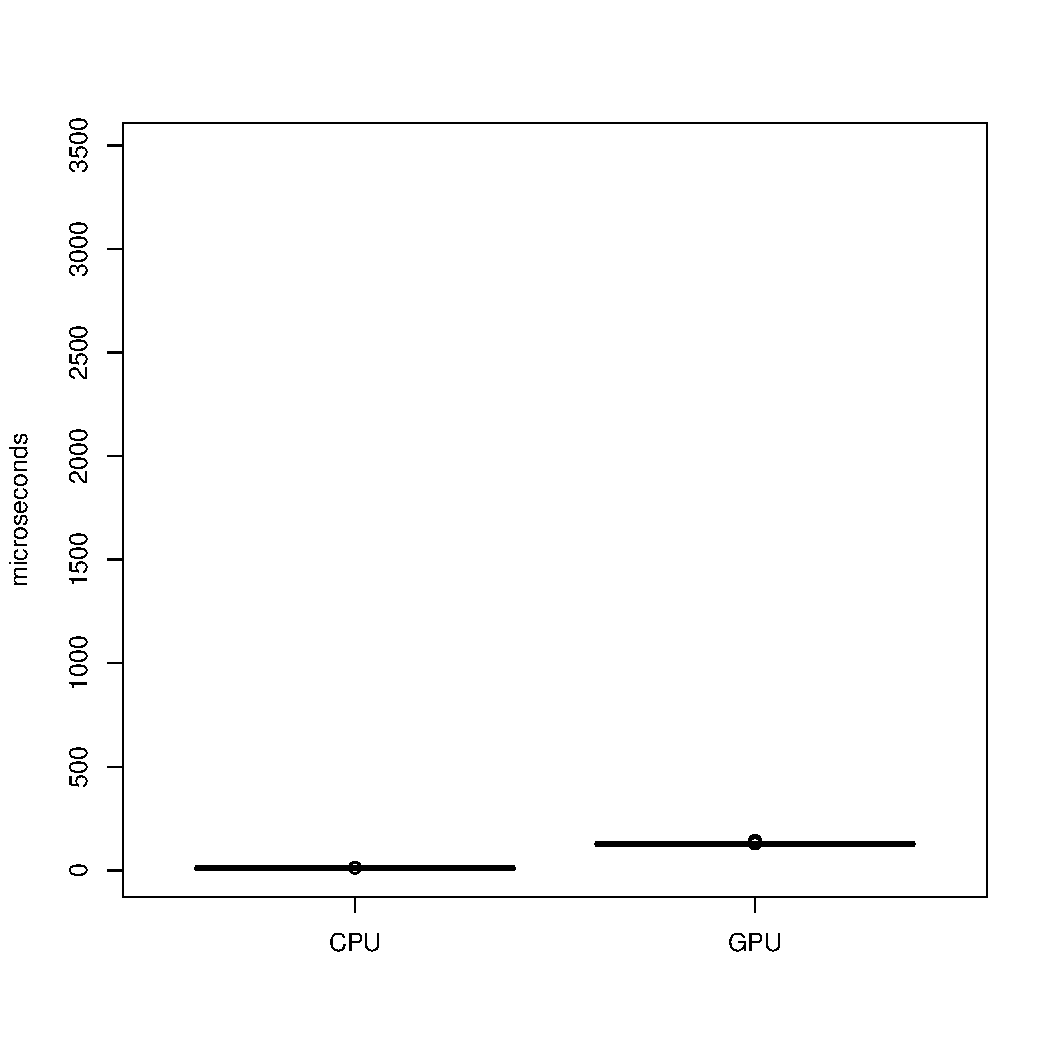
\includegraphics[width=\textwidth]{results/time/sphere_4000}
			\end{subfigure}
			~%
			\begin{subfigure}[b]{0.45\textwidth}
				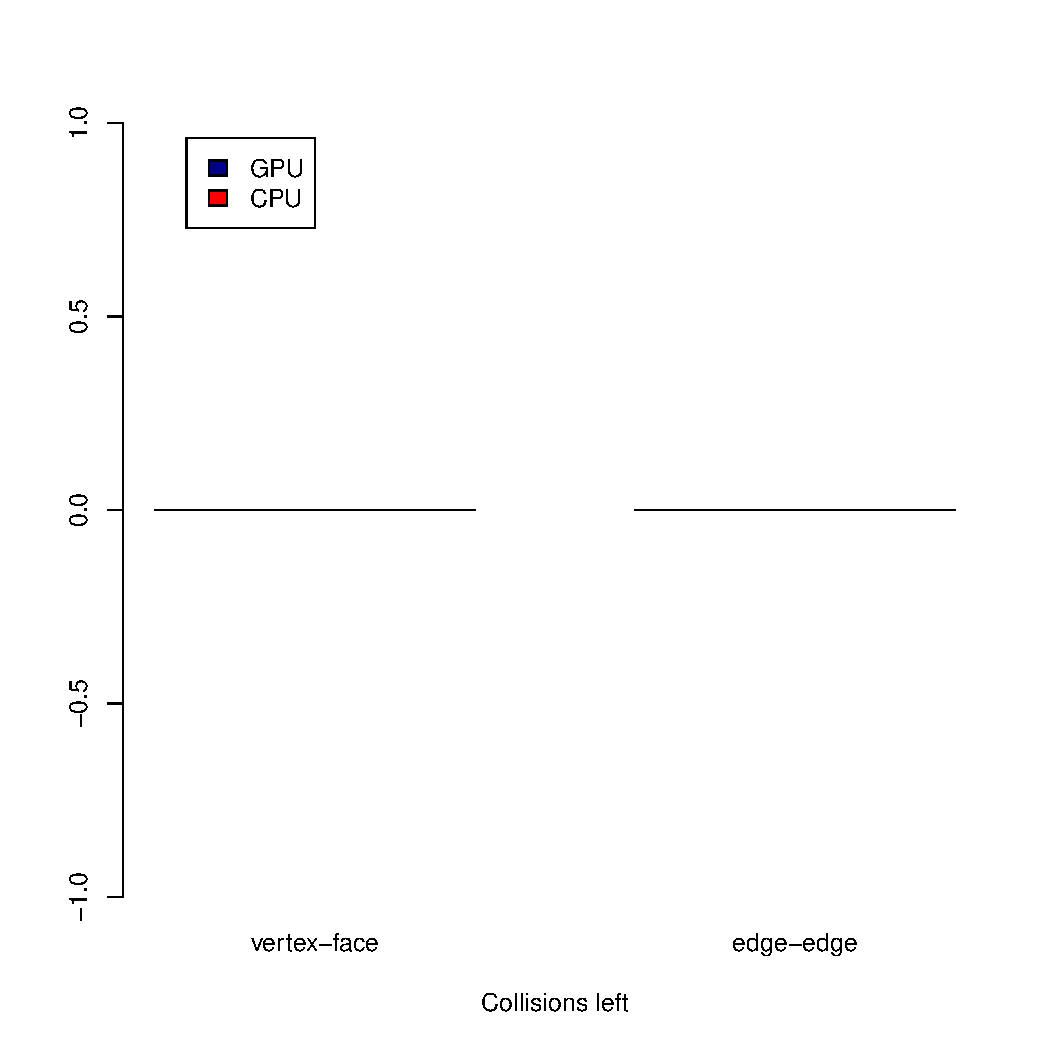
\includegraphics[width=\textwidth]{results/correctness/sphere_4000}
			\end{subfigure}
			\caption{Model \texttt{sphere\_4000.txt}}
		\end{subfigure}
		\caption{Comparison of CPU and GPU versions}
		\label{fig:results}
	\end{figure}
